\documentclass[11pt]{article}
\usepackage[margin=1in]{geometry}
\usepackage{amsmath}
\usepackage{amsfonts}
\usepackage{graphicx}
\usepackage{hyperref}
\usepackage{listings}
\usepackage{xcolor}
\usepackage{natbib}
\usepackage{booktabs}
\usepackage{float}

%R code styling
\lstdefinestyle{Rstyle}{
  language=R,
  basicstyle=\ttfamily\small,
  keywordstyle=\color{blue},
  commentstyle=\color{gray},
  stringstyle=\color{red},
  backgroundcolor=\color{gray!5},
  frame=single,
  breaklines=true,
  showstringspaces=false,
  numbers=left,
  numberstyle=\tiny\color{gray}
}

\title{\textbf{LAVA: Log ratios of Ancestral Variances} \\
       \large A Method for Identifying Local Adaptation in Structured Populations}
\author{Isabela do O, Oscar E Gaggiotti, Pierre de Villemereuil, Jerome Goudet}
\date{\today}

\begin{document}

\maketitle

\begin{abstract}
The LAVA package implements the LogAV method for testing local adaptation in structured populations by comparing log ratios of ancestral variances. The method addresses limitations of traditional $Q_{ST}$-$F_{ST}$ comparisons by accounting for complex population structures through coancestry matrices. The LAVA package implements the LogAV algorithm. This vignette provides a comprehensive guide to using LAVA, including theoretical background, practical examples, and interpretation of results. 
\end{abstract}

\tableofcontents
\newpage

\section{Introduction}

Species are distributed across heterogeneous environments, leading to population divergence through genetic drift, natural selection, and limited gene flow. Distinguishing adaptive divergence from neutral processes is a fundamental challenge in evolutionary biology. Traditional methods like $Q_{ST}$-$F_{ST}$ comparison assume equal relatedness among subpopulations—a simplification that can cause increase in false positive rates [cite de Villemereuil 2020, and do O 2025].

The LAVA package implements the LogAV method [cite do O 2025], which uses estimates of between- and within-population relatedness to model population structure. Under neutrality, the ancestral additive genetic variances estimated from between-population and within-population effects are expected to be equal.

\section{Theoretical Background}

\subsection{The LogAV Method}

LogAV tests the null hypothesis of neutral divergence by comparing two estimates of the ancestral additive genetic variance ($V_A$):

\begin{itemize}
\item $\hat{V}_{A,B}$: estimated from between-population effects
\item $\hat{V}_{A,W}$: estimated from within-population effects
\end{itemize}

Under neutrality: $V_{A,B} = V_{A,W}$

The test statistic is:
$$\text{LogAV} = \log\left(\frac{\hat{V}_{A,B}}{\hat{V}_{A,W}}\right)$$

\subsection{Population structure description}

\subsection{Coancestry Estimation}
We use and recommend the use of the allele-sharing method of moments [cite Weir and Goudet 2017 and Goudet and Weir 2023] to estimate coancestries for using the LAVA package. 

LogAV uses two key matrices:

\subsubsection{Population Coancestry Matrix ($\mathbf{\Theta_p}$)}
$\mathbf{\Theta_p}$ contains mean coancestries for pairs of individuals one in each of two different subpopulations relative to the ancestral population. Element $\Theta_p^{i,j}$ describes the probability of identity-by-descent (IBD) between random alleles from subpopulations $i$ and $j$.

$$\hat{\Theta}_p = \frac{\bar{A}^{\mathcal{P}}_s - \min(\bar{A}^{\mathcal{P}}_s)}{1 - \min(\bar{A}^{\mathcal{P}}_s)}$$

\subsubsection{Individual Coancestry Matrix ($M$)}
$M$ describes relatedness between pairs of individuals within subpopulations, accounting for the shared ancestry already captured in $\Theta_p$.

\subsubsection{Relatedness Adjustment}

Within-population relatedness is adjusted to considering between-population coancestry twice as:

$$\hat{M}_x = \text{relatedness}_x \times (1 - \hat{\Theta}^p_x)$$

where $\hat{\Theta}^p_x$ is the diagonal element of $\hat{\Theta}_p$ for population $x$.


\subsection{Mixed Effects Model}

The phenotypic model is:
$$z \sim \mu + a_p + a_i + \epsilon$$

where:
\begin{align}
a_p &\sim N(0, 2\Theta_p V_{A,B}) \\
a_i &\sim N(0, M V_{A,W})
\end{align}

\section{Installation and Setup}

\lstset{style=Rstyle}
\begin{lstlisting}
# Install from GitHub
devtools::install_github("isadoo/LAVA")

# It automatically installs required dependencies:
# - kinship2 (for kinship calculations)
# - hierfstat (for coancestry estimation)
# - brms (for Bayesian mixed models)
# - JGTeach (for population genetics utilities)
# - gaston (for genetic data manipulation)
# - Matrix (for efficient matrix operations)

library(LAVA)

\end{lstlisting}

\section{Data Requirements}

LAVA requires:

\begin{enumerate}
\item \textbf{Phenotypic data}: Offspring (F1) traits measured in common garden
\item \textbf{Genetic markers}: Genetic markers from founder population (non-common gardens)
\item \textbf{Relatedness for F1}: Pedigree information or genetic markers from F1 individuals(common gardens individuals)
\item \textbf{Population identification}: Founder and F1 individuals should be linked to a population.
\end{enumerate}

\subsection{Data Format}
\begin{itemize}
    \item Genetic data should be in dosage format (0 for reference homozygote, 1 for heterozygote, 2 for derived homozygote), with individuals as rows and loci as columns. with $n$ individuals and $L$ loci, the dosage matrix is $n \times L$.
    \item Population identification for F1 should be a data frame including population names and individual names (dimension $n \times 2$).
    \item Population identification for founder population should be a vector of population names (vector of length $r$ with $r$ populations).
    \item Trait data should be a data frame with at least two columns, one with individual identification and another with trait values (dimension $n \times 2$). 
\end{itemize}

\section{Workflow Overview}

LAVA follows a straightforward workflow:

\begin{enumerate}
\item \textbf{Prepare Data}: Organize genetic markers, phenotypes, and population information
\item \textbf{Calculate Coancestries}: Compute $\Theta_P$ (population-level) and $M$ (individual-level) matrices
\item \textbf{Run Analysis}: Fit the mixed model and estimate ancestral variances
\item \textbf{Interpret Results}: Evaluate evidence for local adaptation
\end{enumerate}

Here we show a general overview of what the steps are. In section (\S\ref{sec:parameters}) we offer a detailed description of the parameters.
On section (\S\ref{sec:tutorial}) we provide a complete tutorial with example data.


\bigskip
\textit{This is not a tutorial, just the description of step-by-step}
\subsection{Step 1: Prepare Your Data}
To run LAVA it is necessary to have coancestries of your populations and measurements of the trait of interest.
We provide a function \texttt{FUNCTION.NAME} to calculate coancestries from genetic data in dosage format. 
To use \texttt{FUNCTION.NAME} you will need genetic data from the populations of origin for example:
\begin{lstlisting}
head(genetic_data_parents)
#   ind_id  pop_id  locus1  locus2  locus3  ...
#   P001    pop1    1       0       2       
#   P002    pop1    0       1       1       
#   P003    pop2    2       2       0       
\end{lstlisting}

You will also need a data frame mapping individuals to populations, with columns specifying individual IDs and population IDs:
\begin{lstlisting}
head(population_ind)
#   id      population_id
#   F001    pop1
#   F002    pop1  
#   F003    pop1
#   F004    pop2
#   F005    pop2
\end{lstlisting}

The last required data entry is the trait data, which should identify individuals and their trait values.
\begin{lstlisting}
head(trait_data)
#   id      trait_value
#   F001    15.2
#   F002    14.8
#   F003    16.1
\end{lstlisting}

To calculate the $\mathbf{M}$ matrix, it is necessary to have either a pedigree data frame or dosages from the F1 (phenotyped) individuals.

\subsection{Step 2: Calculate Coancestries}
Once you have organized your data, you can calculate the coancestry matrices using the \texttt{calculate\_coancestries()} function:
\begin{lstlisting}
# get population IDs for parents
parent_populations <- genetic_data_parents$pop_id

# Calculate coancestry matrices
coancestries <- calculate_coancestries(
  genetic_data_parents = genetic_data_parents[, -c(1:2)], # Remove ID columns
  genotyped_parent_populations = parent_populations,
  genetic_data_F1 = genetic_data_F1[, -c(1:2)], # If available
  population_individual_id = population_ind,
  column_individual = "id",
  column_population = "population_id"
)

# Extract matrices
Theta.P <- coancestries$Theta.P
M <- coancestries$M

# Confirming matrices dimensions
dim(Theta.P)  # Should be n_populations x n_populations
dim(M)    # Should be n_individuals x n_individuals
\end{lstlisting}

\subsection{Step 3: Run LogAV Analysis}
Now you have all the basic requirements to run LAVA.
\begin{lstlisting}
# Run LAVA analysis
result <- lava(
  Theta.P = Theta.P,
  M = M,
  trait_dataframe = trait_data,
  column_individual = "id",
  column_trait = "trait_value"
)

# View results
print(result)
\end{lstlisting}

\subsection{Step 4: Interpret Results}

\begin{lstlisting}
# Plot posterior distributions
plot(result, which = "both")

# Extractstatistics
cat("Mean log ratio:", result$log_ratio$mean_log_ratio, "\n")
cat("P-value:", result$log_ratio$p_value, "\n")
cat("95% CI:", result$log_ratio$log_ratio_ci_lower, 
    "to", result$log_ratio$log_ratio_ci_upper, "\n")
\end{lstlisting}

\section{Function Reference}
\label{sec:parameters}

\subsection{calculate\_coancestries()}

Computes the coancestry matrices required for LAVA.

\begin{lstlisting}
calculate_coancestries(genetic_data_parents,
                       genotyped_parent_populations, 
                       genetic_data_F1 = NA, 
                       population_individual_id = NA, 
                       column_individual = "id", 
                       column_population = "population_id", 
                       pedigree = NA,
                       all_parents_genotyped = FALSE)
\end{lstlisting}

\textbf{Parameters:}

\begin{itemize}
    \item \texttt{genetic\_data\_parents}: Matrix or data frame of genetic data (dosage format: 0, 1, 2) for the parental/founder generation. Individuals in rows, loci in columns.
    
    \item \texttt{genotyped\_parent\_populations}: Vector of population IDs corresponding to rows in \texttt{genetic\_data\_parents}.
    
    \item \texttt{genetic\_data\_F1}: (Optional) Genetic data for F1 generation in dosage format. Default \texttt{NA}.
    
    \item \texttt{population\_individual\_id}: (Optional) Data frame mapping individuals to populations, with columns specified by \texttt{column\_individual} and \texttt{column\_population}. Default \texttt{NA}.
    
    \item \texttt{column\_individual}: Column name for individual IDs in \texttt{population\_individual\_id}. Default \texttt{"id"}.
    
    \item \texttt{column\_population}: Column name for population IDs in \texttt{population\_individual\_id}. Default \texttt{"population\_id"}.
    
    \item \texttt{pedigree}: (Optional) Data frame with columns for individual ID, dam ID, and sire ID. Default \texttt{NA}.
    
    \item \texttt{all\_parents\_genotyped}: Logical; \\
    if \texttt{TRUE}, indicates that the genotyped individuals in \texttt{genotyped\_parent\_populations} are the parents of F1 individuals.\\
    Default is \texttt{FALSE}.
\end{itemize}

\textbf{Returns:} List with components \texttt{Theta.P} (population coancestry matrix) and \texttt{M} (individual relatedness matrix).

\subsection{lava()}

Performs the LogAV analysis to test for local adaptation.

\begin{lstlisting}
lava(Theta.P, 
     M, 
     trait_dataframe, 
     column_individual = "id", 
     column_trait = "trait", 
     formula = "Y ~ 1 + (1 | gr(pop, cov = two.Theta.P)) + (1 | gr(ind, cov = M))", 
     ...)
\end{lstlisting}

\textbf{Parameters:}

\begin{itemize}
    \item \texttt{Theta.P}: Square matrix of population coancestries (from \texttt{calculate\_coancestries()}).
    
    \item \texttt{M}: Square matrix of individual relatedness (from \texttt{calculate\_coancestries()}).
    
    \item \texttt{trait\_dataframe}: Data frame with individual IDs and trait values.
    
    \item \texttt{column\_individual}: Column name for individual IDs. Default \texttt{"id"}.
    
    \item \texttt{column\_trait}: Column name for trait values. Default \texttt{"trait"}.
    
    \item \texttt{formula}: Model formula for \texttt{brms}. Default fits the standard LAVA model.
    
    \item \texttt{...}: Additional arguments passed to \texttt{brms::brm()} (e.g., \texttt{iter}, \texttt{chains}, \texttt{prior}).
\end{itemize}

\textbf{Returns:} LAVA results object with log ratio estimates, credible intervals, and p-values. The fitted \texttt{brms} model is stored as an attribute.

\section{Tutorial: 18 Population Stepping Stones}
\label{sec:tutorial}
Here we show a step by step example of how to run lava on a simple simulated data set.

\subsection{Quick description of our example}

The example dataset comes from a simulated metapopulation:

\begin{itemize}
\item \textbf{Founder populations}: 18 subpopulations in 1-dimensional stepping-stone structure
\item \textbf{Evolutionary history}: 3000 generations in an environmental gradient we refer to as "sine"-like creating selection gradient, as shown in Figure \ref{fig:SSsine}
\item \textbf{Breeding design}: Controlled common garden with a North Carolina II design (add reference)
  \begin{itemize}
  \item Within-population crosses to preserve population structure
  \item Each population split into sires and dams
  \item Multiple offspring per mating pair
  \end{itemize}
\item \textbf{Trait architecture}: Additive genetic model
  \begin{itemize}
  \item 100 quantitative trait loci (QTLs)
  \item Effect size: 0.1 per allele
  \item heritability: $h^2 = 0.8$
  \item Trait centered and standardized
  \end{itemize}
\end{itemize}

\begin{figure}[h!]
    \centering
    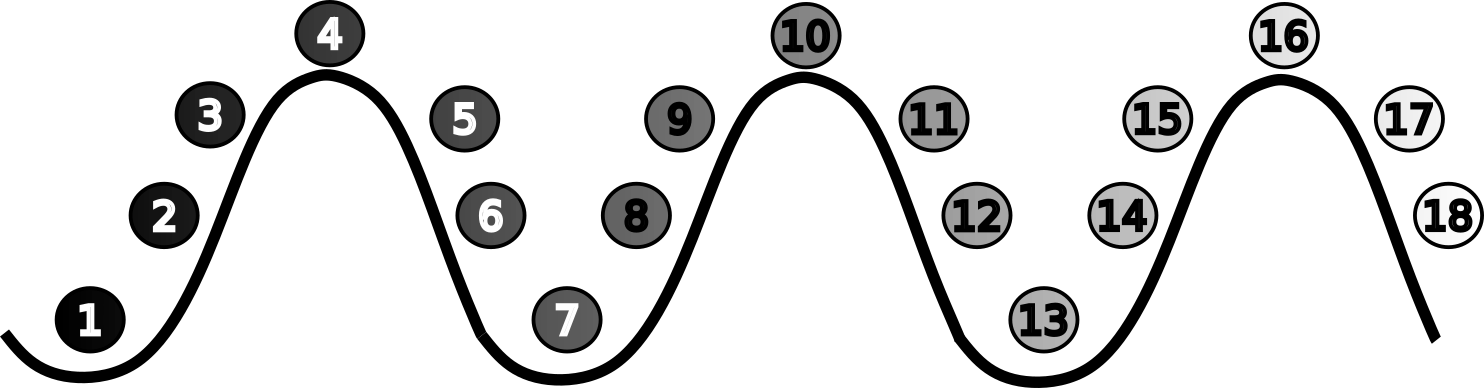
\includegraphics[width=0.8\linewidth]{figures/methods_SS_sine.png}
    \caption{Sine-like environmental gradient across the 18 stepping-stone populations. The figure shows the environmental selection gradient that drove local adaptation in the simulated metapopulation over 3000 generations.}
    \label{fig:SSsine}
\end{figure}

\subsection{Step 1: Load genetic data (neutral markers in dosage format)}

The LAVA package includes example data from a simulated stepping-stone metapopulation. We start by loading the parental (founder) population genetic data and converting it to dosage format:

\begin{lstlisting}
# Load required packages
library(LAVA)
library(hierfstat)

# Read parental population genetic data
neutral_file <- system.file("extdata", "neutral_data_g3000.dat", 
                            package = "LAVA")

sim <- hierfstat::read.fstat(fname = neutral_file)
dos <- hierfstat::biall2dos(sim[, -1])  # Convert to dosage format
pop <- sim$Pop  # Extract population IDs

# View parental dosage data
dos[1:5, 1:5]
#      n1_l1 n1_l2 n1_l3 n1_l4 n1_l5
# [1,]     2     0     1     0     2
# [2,]     2     0     0     0     1
# [3,]     2     0     2     0     2
# [4,]     2     0     0     0     0
# [5,]     2     0     0     0     0

# Check population structure
unique(pop)  # Should show populations 1 through 18
table(pop)   # Individuals per population
\end{lstlisting}

Now load the F1 (common garden) generation neutral markers:

\begin{lstlisting}
# Load F1 generation dosage data
dos_F1only_neutral <- readRDS(
  system.file("extdata", "vignette_dos_F1only_neutral.rds", 
              package = "LAVA")
)

# View F1 dosage data
dos_F1only_neutral[1:5, 1:5]
#      [,1] [,2] [,3] [,4] [,5]
# [1,]    2    0    0    0    1
# [2,]    2    0    1    0    1
# [3,]    2    0    1    0    2
# [4,]    2    0    1    0    1
# [5,]    2    0    1    0    1

dim(dos_F1only_neutral)  # Check dimensions
\end{lstlisting}

\subsection{Step 2: Load trait data and visualize distribution}

Load the trait measurements and population identifications for F1 individuals:

\begin{lstlisting}
# Load trait data
trait_df_pop <- read.csv(
  system.file("extdata", "vignette_trait_df_pop.csv", 
              package = "LAVA")
)

head(trait_df_pop)
#   individual      trait trait_id population
# 1          1 -1.7629615        1          1
# 2          2 -1.6589637        1          1
# 3          3 -1.2060932        1          1
# 4          4 -0.1079098        1          1
# 5          5 -1.5611013        1          1
# 6          6 -1.1595368        1          1

# Load population-individual mapping
population_individual_id_df <- read.csv(
  system.file("extdata", "vignette_population_individual_id_df.csv", 
              package = "LAVA")
)

head(population_individual_id_df)
#   pop_id individual
# 1      1          1
# 2      1          2
# 3      1          3
# 4      1          4
# 5      1          5
# 6      1          6
\end{lstlisting}

Visualize the trait distribution across populations to inspect patterns:

\begin{lstlisting}
# Create visualization
unique_pops <- unique(trait_df_pop$population)
n_pops <- length(unique_pops)
colors <- rainbow(n_pops)

plot(trait_df_pop$individual, trait_df_pop$trait,
     col = colors[as.factor(trait_df_pop$population)],
     pch = 19, cex = 0.8,
     xlab = "Individual ID", 
     ylab = "Trait Value (standardized)",
     main = "Trait Distribution by Population")
legend("topright", legend = paste("Pop", unique_pops), 
       col = colors, pch = 19, cex = 0.8, bty = "n")
\end{lstlisting}

This plot helps visualize population-level trait differences and confirms that traits follow the expected pattern from the selection gradient (Figure \ref{fig:SSsine}).

\subsection{Step 3: Calculate coancestry matrices}

Use the \texttt{calculate\_coancestries()} function to compute the required matrices:

\begin{lstlisting}
coancestries_dosage <- calculate_coancestries(
  genetic_data_parents = dos,
  genotyped_parent_populations = pop,
  genetic_data_F1 = dos_F1only_neutral,
  population_individual_id = population_individual_id_df,
  column_individual = "individual",
  column_population = "pop_id",
  all_parents_genotyped = TRUE,
  verbose = TRUE
)
# There are 18 populations.
# Calculating Theta.P
# Theta.P calculated with dimensions 18 18
# Calculating M
# population sizes of F1 50 50 50 50 50 50 50 50 50 50 50 50 50 50 50 50 50 50
# total individuals are 900
# M calculated with dimensions 900 900

# Extract the matrices
Theta.P <- coancestries_dosage$Theta.P
M <- coancestries_dosage$M

# Verify dimensions
dim(Theta.P)  # [1] 18 18  (populations x populations)
dim(M)        # [1] 900 900  (individuals x individuals)
\end{lstlisting}

\subsection{Step 4: Run LAVA analysis}

Now we can run the LAVA analysis using the coancestry matrices and trait data:

\begin{lstlisting}
results <- lava(
  Theta.P = Theta.P,
  M = M,
  trait_dataframe = trait_df_pop,
  column_individual = "individual",
  column_trait = "trait",
  save_full_model = FALSE,  # Save memory
  iter = 4000,           
  warmup = 2000,         
  control = list(adapt_delta = 0.95, max_treedepth = 12)
)
\end{lstlisting}

\subsection{Step 5: Interpret results}

View a concise summary of the results:

\begin{lstlisting}
summary(results)

# === LAVA Summary ===
# 
# Trait: trait
# 
# Log-Ratio of Ancestral Variances (log(VB/VA)):
#   Mean:    1.2345
#   Median:  1.2234
#   95% CI: [0.8765, 1.6789]
#   P-value: 0.0012 *
\end{lstlisting}

For detailed output including convergence diagnostics:

\begin{lstlisting}
print(results)

# === LAVA Analysis Results ===
#
# Trait analyzed: trait
# Formula used: Y ~ 1 + (1 | gr(pop, cov = two.Theta.P)) + ...
#
# --- Log-Ratio of Ancestral Variances ---
#   Mean: 1.2345
#   Median: 1.2234
#   95% Credible Interval: [0.8765, 1.6789]
#   P-value: 0.0012
#
# --- Convergence Diagnostics ---
#   Max R-hat: 1.00 (OK)
#   Divergent transitions: 0 (OK)
\end{lstlisting}

Examine the posterior samples (now showing V\_AB and V\_AW columns):

\begin{lstlisting}
head(results$sampling)
#   b_Intercept sd_pop__Intercept sd_ind__Intercept  V_AB   V_AW log_ratio
#1     -0.00658             0.752             0.410 0.566  0.168      1.22
#2     -0.19000             0.672             0.355 0.452  0.126      1.27
#3      0.24400             0.960             0.391 0.922  0.153      1.80
#4      0.37500             1.200             0.368 1.430  0.135      2.36
#5     -0.20000             0.686             0.363 0.471  0.132      1.27
#6      0.39900             0.835             0.366 0.697  0.134      1.65
\end{lstlisting}

Where:
\begin{itemize}
\item \texttt{V\_AB}: Ancestral variance estimated from between-population effects
\item \texttt{V\_AW}: Ancestral variance estimated from within-population effects  
\item \texttt{log\_ratio}: $\log(V_{AB}/V_{AW})$, the test statistic
\end{itemize}

Visualize the posterior distribution:

\begin{lstlisting}
plot(results)
\end{lstlisting}

\subsection{Interpretation}

In this example:
\begin{itemize}
\item The mean log-ratio is significantly greater than zero ($p < 0.05$)
\item $V_{AB} > V_{AW}$, indicating that between-population variance exceeds within-population variance after accounting for population structure
\item This provides evidence for \textbf{local adaptation}: populations have diverged more than expected under neutral evolution
\item The 95\% credible interval does not include zero, supporting this conclusion
\end{itemize}

A positive log-ratio suggests that selection has caused greater differentiation between populations than drift alone would produce. The magnitude of the effect can be interpreted from the posterior distribution of the log-ratio.
\section{Advanced Topics}
\subsection{Pick your prior}
As it should be clear by now, the \texttt{lava()} function uses Bayesian inference through the \texttt{brms} package, and is through it that the ancestral variances are estimated. Thus, it requires you to specify a \textbf{prior}; the probability distribution that will describe the prior beliefs about your parameters. 
We rely on the default priors from the brms package that should be sensible for most use cases and which we verified result in a calibrated test in our trials of the method.

\subsection{Common questions}

\begin{enumerate}
\item Can the same dosage data be used to calculate \textbf{M} and $\mathbf{\Theta}^P$? Ideally not. $\mathbf{\Theta}^P$ should describe the relatedness the neutral structure of the populations we are comparing. When we expose F1 to our common gardens we are likely reducing the effect of selection and increasing the effects of drift from separating the populations and from introduced sampling variance. We note on our discussion, there are ways to reconstruct the parental genotypes and thus get $\mathbf{\Theta}^P$ from only sampling genetic data of the common gardens populations. And as reviewer 2 pointed out given reliable ways of estimating the amount of drift between the founder population and the common gardens generation, the issue would be ameliorated
\item Is it necessary to use common gardens? We advise to always use a strategy to standardize the environmental effects over phenotypic measurements. Similarly to the classical framework of $Q_{ST}$--$F_{ST}$ comparison, our method will be impacted by confounding effects of the environment (through phenotypic plasticity) and, even more problematically, by genotype-by-environment interactions. 
\end{enumerate}

\section{Getting Help}

\begin{itemize}
\item Package documentation: \texttt{help(package = "LAVA")}
\item Function help: \texttt{?lava}, \texttt{?calculate\_coancestries}
\item GitHub repository: \url{https://github.com/isadoo/LAVA}
\item GitHub issues: \url{https://github.com/isadoo/LAVA/issues}
\item Contact: isabela.doo@unil.ch
\item Using kinship2 instead of our own function, see \texttt{KINSHIP2\_MIGRATION.md} in the package documentation
\end{itemize}


\bibliographystyle{plainnat}
\bibliography{references}

\appendix

\section{Example usage with real data}
\begin{lstlisting}
data("stickleback_example") # Hypothetical dataset

# Morphological traits
morphological_traits <- c("standard_length", "body_depth", 
                         "head_length", "pelvic_girdle_length")

# Behavioral traits  
behavioral_traits <- c("aggression", "risk_taking")

# Analyze each trait
morph_results <- lapply(morphological_traits, function(trait) {
  lava(Theta.P = stickleback_Theta.P,
       M = stickleback_M,
       trait_dataframe = stickleback_traits,
       column_trait = trait)
})
names(morph_results) <- morphological_traits

# Summary table
results_table <- data.frame(
  Trait = names(morph_results),
  Mean_LogRatio = sapply(morph_results, function(x) x$log_ratio$mean_log_ratio),
  P_value = sapply(morph_results, function(x) x$log_ratio$p_value),
  Significant = sapply(morph_results, function(x) x$log_ratio$p_value < 0.05)
)

print(results_table)
\end{lstlisting}
\section{Example Output}

\begin{verbatim}
===============================
Log Ancestral Variance Analysis (LAVA)
===============================

Log ratio of estimated ancestral variances (between equation/ within equation):
  Mean: 2.1483 (95% CI: 0.8542 to 3.4421)

Difference in variance components (between equation/ within equation):
  Mean: 0.3421
  Median: 0.3387 (95% CI: 0.1234 to 0.5612)

Statistical tests:
  Hypothesis test p-value: 0.0285

===============================
\end{verbatim}

\end{document}